% -*- coding: UTF-8 -*-
% hurlex-chapt9.tex
% hurlex 开发文档 第9章内容

\section {物理内存管理的实现}

\par 这章我们来讨论操作系统内核的一个很重要的组成部分——内存管理模块。之前的章节中简单介绍了段式的内存管理,这章我们来讨论\allowbreak
页式的内存管理。

\par 首先是CPU在保护模式下分页未开启和分页开启的不同状态时,MMU组件处理地址的流程。

\begin{mdframed}
	\begin{itemize}
		\item 如果没有开启分页:\\ 逻辑地址 -> 段机制处理 -> 线性地址 = 物理地址
		\item 如果开启分页:\\ 逻辑地址 -> 段机制处理 -> 线性地址 -> 页机制处理 -> 物理地址
	\end{itemize}
\end{mdframed}

\par 因为采用了平坦模式,所以给出的访问地址实际上已经等于线性地址了(段基址为0),那么剩下的问题就是所谓的页机制处理了。

\par 长时间以来,随着计算机技术的发展,存储器的容量在不断的高速增加着。但是说起内存(这里指RAM,下同)这个东西,\allowbreak
它有一个很奇葩的特性,就是无论它有多大,都总是不够用(P.S.厨房的垃圾桶也一样)。现在我们看似拥有着以前的程序员\allowbreak
想都不敢想的"天文数字"的内存,动辄就是几G十几G的。但是相信我,历史总是嘲弄人的。就像当年程序员们质疑32位地址线带来\allowbreak
的4GB空间太大没有意义似的,我们也会有一天抱怨现在的内存太小的。

\par 那么,既然内存总是不够用的,那内存不够用了怎么办?还有,使用过程中出现的内存碎片怎么办?假设我们有4GB的物理内存,\allowbreak
现在有1、2、3、4一共4个程序分别各占据连续的1G内存,然后2、4退出,此时虽然有空闲的两段内存,却连一个稍大于1GB的程序都无法载入了。

\par 当然了,这只是一个例子。不过按照一般的思路,在内存释放之后,如何回收呢?做碎片整理吗?即便我们不在乎整理过程带来的\allowbreak
效率损失,光是程序加载时候的地址逐一重定位就是及其麻烦的。那怎么办?当然了,解决的办法是有的,聪明的计算机工程师们想到了采用\allowbreak
分页的方式来管理物理内存。他们在逻辑上把内存划分为定长的物理页,同时将一个程序执行时候的线性地址地址空间划分为逻辑页,在分页\allowbreak
机制工作的前提下,给硬件提供一组数据结构来保存这种映射关系。也就是说,线性地址是连续的,但是其实际指向的物理地址就不见得是\allowbreak
连续的了。别忘了,RAM是随机存储器,读取任意一个地址的理论时间都是一样的(暂时让我们忘了cache吧)。我们让CPU在寻址的时候,自动\allowbreak
去查找线性地址到物理地址的映射关系,从而找到实际的数据就好。严格说地址翻译是由MMU组件来进行的,但是现在MMU一般都是CPU的一个\allowbreak
组成部分了,所以也就不严格区分了。

\par 下面的图片描述了这个映射关系:

\begin{figure}[H]
      \centering
      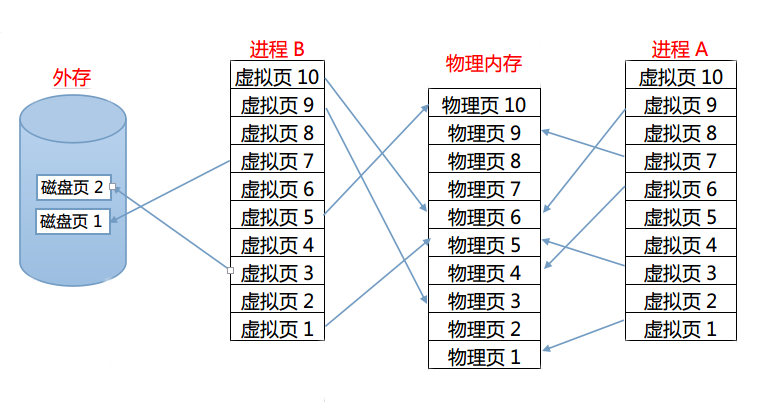
\includegraphics[scale=0.35]{picture/chapt9/PAGE_MAP.png}
      \caption{分页映射}
\end{figure}

\par 一图胜千言,我们看到了固定大小的物理页、虚拟页、甚至还有磁盘页。我觉得这张图片很能说明问题了,相信聪明的你从这里都悟出\allowbreak
来了虚拟内存的实现原理了。没错,虚拟内存实质上就是把物理内存中暂时用不到的内容暂时换出到外存里,空出内存放置现阶段需要的数\allowbreak
据。至于替换的策略当然有相应的算法了,比如最先换入原则,最少使用原则等等方法可以使用。

\par 相信通过上文的描述,我们对分页已经建立了初步的理解了。那么接下来的问题是,怎么表示和存储这个映射关系。这里描述起来简单,\allowbreak
但是代码就不是那么直观了,原因很简单,因为需要一组数据结构来管理内存,但是这组数据结构本身也得放在内存里。所以牵扯到一个自\allowbreak
己管理自己的问题。而且,开启分页模式之后,CPU立即就会按照分页模式的规则去解释线性地址了。所以,这意味着必须先建立好地址映射\allowbreak
的数据结构,才能开启分页,而且必须保证之前的代码地址和数据地址都能映射正确。

\par 下面我们来说说x86下的一种简单的做法吧。

\par 在32位操作系统下使用32位地址总线(暂时原谅我在这里错误的描述吧,其实还有PAE这个东西),所以寻址空间有2的32次方,也就\allowbreak
是4GB。一定要注意,我们强调了很多次了,这个空间里,有一些断断续续的地址实际上是指向了其它的外设,不过大部分还是指向RAM的。\allowbreak
具体采取的分页大小可以有多种选择,但是过于小的分页会造成管理结构太大,过于大的分页又浪费内存。现在较为常见的分页是4KB一个页,\allowbreak
也就是4096字节一个页。简单计算下,4GB的内存分成4KB一个的页,那就是1MB个页,没错吧?每个虚拟页到物理页的映射需要4个字节来\allowbreak
存储的话(别忘了前提是32位环境下),整个4GB空间的映射需要4MB的数据结构来存储。

\par 目前看起来一切都很好,4MB似乎也不是很大。但是,这只是一个虚拟地址空间的映射啊,别忘了每个进程都有自己的映射,而且\allowbreak
操作系统中通常有N个进程在运行。这样的话,假如有100个进程在运行,就需要400MB的内存来存储管理信息!这就太浪费了。

\par 怎么办?聪明的工程师们提出了分级页表的实现策略,他们提出了页目录,页表的概念。以32位的地址来说,分为3段来寻址,分别是\allowbreak
地址的低12位,中间10位和高10位。高10位表示当前地址项在页目录中的偏移,最终偏移处指向对应的页表,中间10位是当前地址在该页表\allowbreak
中的偏移,我们按照这个偏移就能查出来最终指向的物理页了,最低的12位表示当前地址在该物理页中的偏移。就这样,我们就实现了分级页表。

\par 我们来张图看看:

\begin{figure}[H]
      \centering
      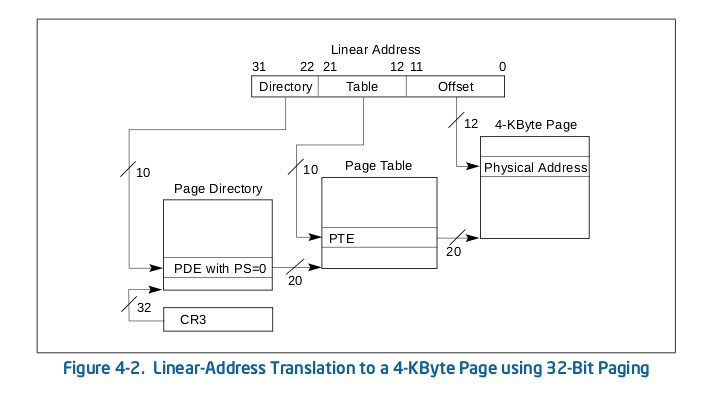
\includegraphics[scale=0.5]{picture/chapt9/PAGE.png}
      \caption{多级页表}
\end{figure}

\par 也许你已经算出来了,这样做的话映射4GB地址空间需要4MB+4KB的内存。我们这是搬起石头砸了自己的脚吗?当然不是,\allowbreak
因为在一个进程中,实际使用到的内存大都远没有4GB这么大,所以通过两级页表的映射,我们就可以只映射需要的地址就可以了,\allowbreak
是不是节省了内存呢?概念我们暂时就说到这里,更专业的描述和规范请参阅Intel文档,也就是上面那张图片的出处。

\par 说完了理论,接下来就是具体的实现了。我们把内存管理分为物理内存管理和虚拟内存管理两个部分来进行。本章讨论物理内存的管理。\allowbreak
要实现内存的管理,首先要解决以下三个问题:

\begin{mdframed}
	\begin{enumerate}
		\item 如何获取可用物理内存的大小和地址?
		\item 采用什么样的数据结构来描述物理内存?
		\item 申请和释放物理内存的算法如何实现?
	\end{enumerate}
\end{mdframed}

\par 我们先来解决第一个问题。获取物理内存的方法一般有BIOS调用和直接探测等方法,但是GRUB的Mutliboot协议提供了更简单的方法。\allowbreak
还记得那个multiboot\_t结构体吗?GRUB已经获取了物理内存的分布并且把它们放置在了这个结构体里的以下两个成员里。

\begin{lstlisting}[language = C, caption = include/multiboot.h]
typedef
struct multiboot_t {
	
	... ...

	/**
	 * 以下两项指出保存由 BIOS 提供的内存分布的缓冲区的地址和长度
	 * mmap_addr 是缓冲区的地址, mmap_length 是缓冲区的总大小
	 * 缓冲区由一个或者多个下面的 mmap_entry_t 组成
	 */
	uint32_t mmap_length;		
	uint32_t mmap_addr;
	
	... ...

} __attribute__((packed)) multiboot_t;

/**
 * size 是相关结构的大小,单位是字节,它可能大于最小值 20
 * base_addr_low 是启动地址的低32位,base_addr_high 是高 32 位,启动地址总共有 64 位
 * length_low 是内存区域大小的低32位,length_high 是内存区域大小的高 32 位,总共是 64 位
 * type 是相应地址区间的类型,1 代表可用 RAM,所有其它的值代表保留区域
 */
typedef
struct mmap_entry_t {
	uint32_t size; 		// size 是不含 size 自身变量的大小
	uint32_t base_addr_low;
	uint32_t base_addr_high;
	uint32_t length_low;
	uint32_t length_high;
	uint32_t type;
} __attribute__((packed)) mmap_entry_t;
\end{lstlisting}

\par GRUB将内存探测的结果按每个分段整理为mmap\_entry结构体的数组。mmap\_addr是这个结构体数组的首地址,mmap\_length是整个数组的长度。

\par 这里需要留意的是mmap\_entry结构体的size成员指的是除了size之外的成员的大小。至于base和length拆为了两段是因为物理地址\allowbreak
可能用32位表示不下,不过我们只考虑32位操作系统,而且暂时只支持512MB的内存即可。type成员用来描述这个内存段的属性,因为物理\allowbreak
不一定指向RAM里,也可能是其它外设。

\par 现在第一个问题解决了一半了,但是我们需要知道内核本身加载到物理内存的位置信息,这块内存必须是管理区域被保留的。\allowbreak
怎么获取呢?看起来很困难,其实解决起来特别容易。大家想想,链接器负责了整个内核文件的链接和重定位工作,肯定知道内核\allowbreak
文件加载到内存中的位置。我们修改链接器脚本,定义两个变量:

\begin{lstlisting}[caption = script/kernel.ld]
	... ...
	
	/* 代码段起始位置 */
	.text 0x100000 :
	{
		PROVIDE( kern_start = . );
		code = .; _code = .; __code = .;
		*(.text)
		. = ALIGN(4096);
	}

	... ....

	.stabstr :
	{
		stabstr = .; _stabstr = .; __stabstr = .;
		*(.stabstr)
	 	. = ALIGN(4096);
		PROVIDE( kern_end = . );
	}
	
	... ...
\end{lstlisting}

\par 我们在最先放置的段.text的开始位置和最后一个段.stabstr的结尾定义了两个变量kern\_start和kern\_end,这两个变量\allowbreak
在C代码里声明后就可以了。

